\subsection{Le Modele - Vue - Controlleur}

La première idée que nous avons eu a été d'introduire un desgin pattern afin de structurer l'architecture globale de l'application. \\ Le pattern MVC permet en effet de découper l'application en trois grandes parties :
\begin{itemize}
 	\item l'affichage de données (Vue)
 	\item la sauvegarde et manipulation de données (Modele)
 	\item la gestion des interactions de l'utilisateur (Controlleur)
 \end{itemize}
Nous avons donc adapté le MVC à notre application dont voici le diagramme de classe : \\[0.5cm]
\centerline{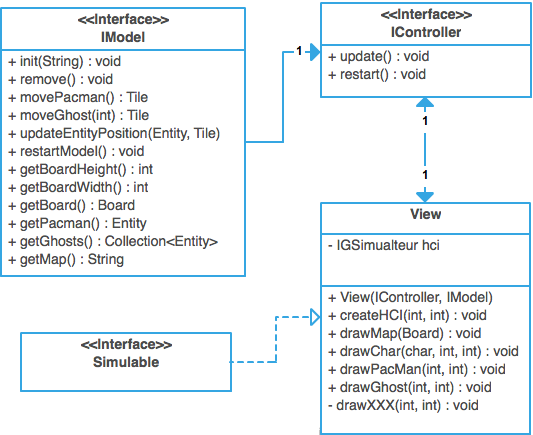
\includegraphics[scale=0.5]{MVC}}

En suivant la logique de ce diagramme de classe, nous remarquons que le controller ne possède que deux méthodes. En effet, nous avons à gérer deux types d'évènement : l'avancement de la simulation gérée par la méthode update() et la remise à zéro de la simulation (restart()).
Afin de détailler une des deux méthodes, prenons l'exemple de la mise à jour :

\begin{lstlisting}
/* DANS LA VUE */
public void next() {
	controller.update();
}

/* DANS LE CONTROLLEUR */
//Methode update
public void update () {
	updatePacman();
	updateGhosts();
}

//Methode updatePacman
private void updatePacman() {
	Tile tile = this.model.getPacman().getPosition();
	Tile newTilePM = this.model.movePacman();
	this.model.getPacman().setPosition(newTilePM);
	this.model.updateEntityPosition(this.model.getPacman(), tile);
	view.drawPacMan(newTilePM.getX(), newTilePM.getY());
	view.drawSpace(tile.getX(), tile.getY());
}
\end{lstlisting}
Lorsque l'utilisateur appuie sur le bouton next sur l'IHM, la méthode next() de la vue est appelée. La vue fait alors appel à son controller qui devra gérer cette évènements. \\
Dans ce cas, la méthode update() du controller a pour rôle de mettre à jour Pacman et les fantômes. En se penchant sur la mise à jour de Pacman, nous voyons le mécanisme de déplacement d'un personnage. Nous récupérons la case courante, puis le modele se charge de calculer la nouvelle position du personnage, se fait ensuite l'attribution de cette nouvelle position. La partie gestion des données est finie, il ne reste qu'à déléguer l'affichage à la vue. Les méthodes de dessin de la vue se servent de l'objet simulable. Quant au modele, le calcul des postions est délégué au personnage (voir la partie gestion de personnage ci-après). Son principal rôle est de stocker les données et de les maintenir à jour à chaque tour. Son second rôle est aussi de parser les fichiers de cartes et créer les données associées.




